\normaltrue \difficilefalse \tdifficilefalse
\correctionfalse
%\UPSTIidClasse{11} % 11 sup, 12 spé
%\newcommand{\UPSTIidClasse}{11}

\exer{Roburoc$\star$ \label{CHS:03:B2:16:79}}
%% 
\setcounter{question}{0}\marginnote{\xpComp{CHS}{03}}%\UPSTIcompetence[2]{B2-16}
\index{Compétence CHS-03}\index{Compétence B2-16}

\index{Roburoc}
\index{Hyperstatisme}

\ifcorrection
\else
\marginnote{\textbf{Pas de corrigé pour cet exercice.}}
\fi


\ifprof
\else
On s'intéresse au roburoc, une plateforme exploratrice tout terrain.


\begin{figure*}[!h]
\centering
\begin{subfigure}[c]{.23\linewidth}
\centering
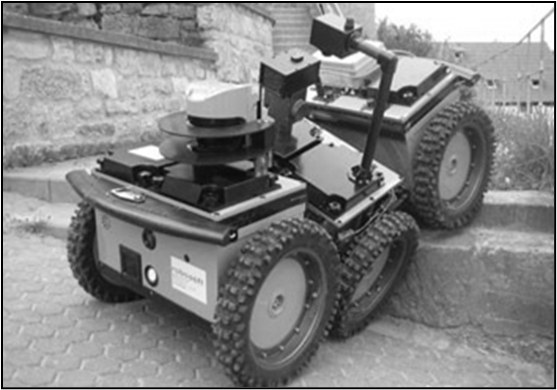
\includegraphics[height=3cm]{79_01.png}
\end{subfigure} \hfill
\begin{subfigure}[c]{.23\linewidth}
\centering
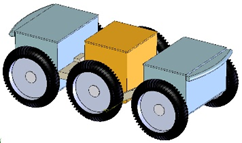
\includegraphics[height=3cm]{79_02.png}
\end{subfigure} \hfill
\begin{subfigure}[c]{.23\linewidth}
\centering
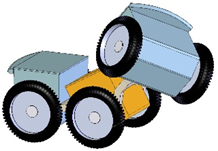
\includegraphics[height=3cm]{79_03.png}
\end{subfigure} 
\begin{subfigure}[c]{.23\linewidth}
\centering
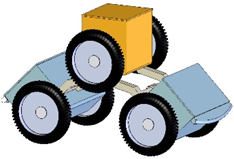
\includegraphics[height=3cm]{79_04.png}
\end{subfigure}
\end{figure*}




\begin{marginfigure}
\centering
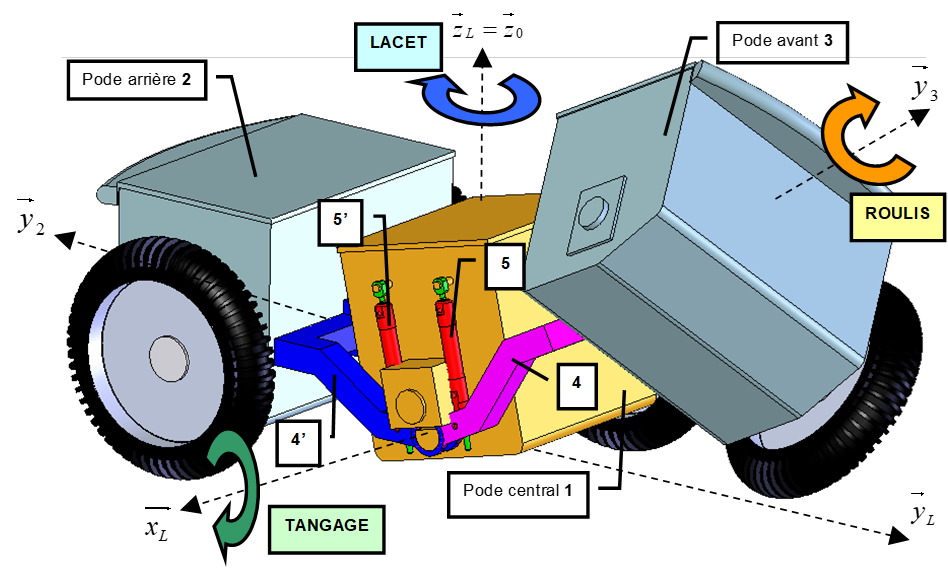
\includegraphics[width=\linewidth]{79_05.png}
%\includegraphics[width=.45\linewidth]{77_02.png}
%\caption{Pince utilisée sur le système ROBOVOLC et schéma cinématique associé \label{fig_23}}
\end{marginfigure} 
\fi


\question{Réaliser le graphe de liaisons.}

\question{Calculer le degré d'hyperstatisme.}

\question{Si le modèle est hyperstatique, modifier le modèle pour le rendre isostatique.}
 

\ifprof
\else

%\noindent\footnotesize
% \fbox{\parbox{.9\linewidth}{
% Éléments de corrigé : 
% \begin{enumerate}
%\item .
%%\item $h=8$.
%\item .
% \end{enumerate}}}
%\normalsize

\marginnote{Corrigé  voir \ref{CHS:03:B2:16:79}.}

\fi